\documentclass[tc,twoside]{iiufrgs} 
\usepackage[T1]{fontenc}        % pacote para conj. de caracteres correto 
\usepackage[utf8]{inputenc}   % pacote para acentua\c c\~ ao 
\usepackage{graphicx}           % pacote para importar figuras 
\usepackage{times}              % pacote para usar fonte Adobe Times 
\usepackage{multirow} 
\usepackage{subfigure} 
\usepackage{listings} 
\usepackage{scalefnt} 
\usepackage[brazilian]{babel} 
\usepackage{tabularx} 
\usepackage{verbatim}
%\usepackage{hyperref} 
%\usepackage{float} 

\bibliographystyle{abnt} 
%\bibliographystyle{apalike} 

\hyphenation{en-si-na-men-tos a-gra-de-ci-men-to de-se-nha-dos} 

\title{Alocação espacial de aparelhos de distribuição de redes IEEE 802.11 em ambientes internos 2D} 

\author{Nunes}{Laura Troina} 

\advisor[Prof. ]{Betito}{Rafael} 

\date{Julho}{2017} 

\location{Rio Grande}{RS} 

\renewcommand{\nominata}{ 
	Instituto Federal de Educação, Ciência e Tecnologia do Rio Grande do Sul\\ 
	Reitor: Prof. Osvaldo Casares Pinto\\ 
	Pró-Reitor de Graduação: Prof. Clarice Monteiro Escott\\ 
	Coordenador do curso: Prof. Rafael Betito\\ 
} 

\keyword{rede sem fio, otimização de cobertura, heuristica, hillclimbing, algoritmo genetico} 

\begin{document} 

\maketitle 

\begin{folhadeaprovacao} 
	Monografia sob o título \textit{"Alocação espacial de aparelhos de distribuição de redes IEEE 802.11 em ambientes internos 2D"}, defendida por Laura Troina Nunes e aprovada em XX de julho de 2017, em Rio Grande, estado do Rio Grande do Sul, pela banca examinadora constituída pelos professores: 
\assinatura{Prof. Rafael Betito\\Orientador} 
\assinatura{Prof. Mscº Luciano Vargas\\Instituto Federal de Educação Ciência e Tecnologia do Rio Grande do Sul}
\assinatura{Prof. Drª Raquel Barbosa\\Instituto Federal de Educação Ciência e Tecnologia do Rio Grande do Sul}  
\end{folhadeaprovacao} 

\clearpage 

\begin{flushright} 
	\mbox{}\vfill 
	{\sffamily\itshape 
		"Do or do not. There is no try."\\} 
	--- \textsc{Mestre Yoda} 
\end{flushright} 
\begin{flushright} 
	\mbox{}\vfill 
	{\sffamily\itshape 
		"Stay hungry. Stay foolish"\\} 
	--- \textsc{Steve Jobs} 
\end{flushright} 
\chapter*{Agradecimentos} 

AGRADECIMENTOS

\tableofcontents 

\begin{listofabbrv}{SPMD} 
	\item[HTTP] protocolo de transferência de hipertexto (\textit{hypertext transfer protocol}) 
	\item[AG] algoritmo genético
	\item[AP] \textit{access point}
\end{listofabbrv} 

\listoffigures 

\listoftables 

\begin{abstract} 
RESUMO
\end{abstract} 

\chapter{Introdução} 

Atualmente, o computador é uma ferramenta fundamental para a realização de tarefas corriqueiras. Com o tempo, eles foram conectados entre si de modo a formar uma rede de informações. Além de cabos, estas redes podem ser montadas através de aparelhos que emite sinais sem fio. Redes sem fio são práticas, pois permitem a conexão de aparelhos sem a limitação de um cabo. Junto dos emissores \textit{wireless}, surgiu também o problema da cobertura de sinal. É normal encontrarmos locais onde apesar de o sinal estar disponível, é impossível navegar através dele. Isso se deve ao mau planejamento do posicionamento dos emissores.

Um exemplo desse problema é a figura \ref{fig:problemaCobertura}. Ela mostra vários aparelhos emissores de sinal sem fio e a cor de cada região representa a qualidade do sinal em cada espaço da planta. As zonas vermelhas são as de maior intensidade do sinal, as amarelas de intensidade média, as verdes de baixa intensidade e as zonas azuis são zonas onde praticamente não existe sinal. 

\begin{figure}[h]
\centering
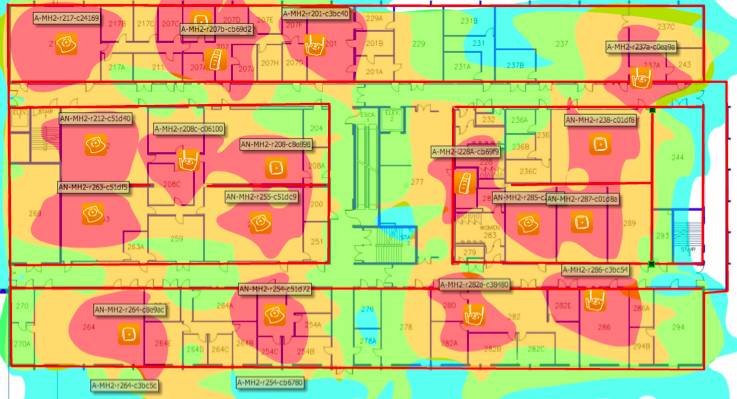
\includegraphics[scale=0.5]{img/problemaCobertura.png}
\caption{Exemplo de distribuição de sinal sem fio}
Fonte: http://gotoitsupport.com/other-it-services/consulting-services/wireless-network-site-surveys/
\label{fig:problemaCobertura}
\end{figure}

Utilizando modelos de propagação de sinal e características do ambiente, serão realizados experimentos com algoritmos genéticos, simulando o posicionamento dos equipamentos de distribuição do sinal \textit{wireless} no interior dos locais alvo, para encontrar o posicionamento de melhor custo benefício.

Esse trabalho tem como objetivo geral otimizar o posicionamento dos aparelhos de espalhamento de sinal \textit{wireless} em uma planta baixa de forma a obter total cobertura com qualidade na troca de dados. Para isto, será necessário o estudo de redes sem fio e tipos de propagação de sinais, estudo das soluções de problemas similares, análise das ferramentas existentes, projeto da solução, validação e testes e por fim aplicação em casos de testes hipotéticos.

 

\chapter{Fundamentação Teórica} 

\section{Redes de Computadores}

Com a popularização do computador, os trabalhos são realizados por um grande número de computadores independentes, porém conectados entre si, formando uma rede. \cite{tanenbaum2003redes} %conferido

Uma rede de computadores é um conjunto de computadores autônomos interconectados por uma tecnologia. Dois computadores são ditos conectados quando estes podem trocar informações. \cite{tanenbaum2003redes} %conferido

As redes são classificadas de acordo com a abrangência geográfica. Redes locais conectam computadores próximos. Redes metropolitanas conectam computadores e redes locais. Redes globais conectam redes metropolitanas. \cite{tanenbaum2003redes} %conferido%

Em uma rede de computadores são utilizados vários protocolos, topologias, métodos de acesso e meios de propagação do sinal. \cite{brisa1997redes} %conferido

\subsection{Redes Não Cabeadas}

Redes sem fio ou também chamadas redes \textit{wireless}, estão cada dia mais populares por serem práticas e proporcionarem mobilidade ao usuário. Nos últimos anos houve um aumento expressivo tanto da qualidade do serviço quanto do número de equipamentos compatíveis. \cite{rappaport2009comunicacoes} %conferido

Esse tipo de rede utiliza sinais de radiofrequência ou infravermelho para a conexão dos usuários e pode ser utilizada em qualquer ambiente. Está sendo cada vez mais utilizada como uma extensão ou alternativa às redes locais cabeadas por prover vantagens econômicas, mobilidade aos usuários, facilidade de instalação e manutenção. \cite{sanches2005projetando} \cite{torres2015redes} %conferido

Quanto ao local de instalação, redes sem fio são classificadas em redes de ambientes internos e externos. Em ambientes internos os equipamentos utilizados são de baixa potência para uma cobertura limitada e distâncias curtas. Em ambientes externos, os equipamentos necessitam de maior potência para proporcionar maior alcance com cobertura ampla ou restrita. É importante ressaltar que em ambas as situações, o sinal da rede sofre atenuações devido às características do ambiente e dos obstáculos encontrados no caminho. \cite{rappaport2009comunicacoes} %conferido

Dentre os equipamentos utilizados para distribuir o sinal sem fio, o mais comum é o ponto de acesso ou \textit{access point}. São eles que possibilitam expandir a infraestrutura da rede se conectando diretamente à rede cabeada ou à outros pontos de acesso. Eles são os responsáveis por gerenciar parâmetros de cada uma das redes e também pela comunicação com os clientes sem fio através dos padrões IEEE 802.11. São equipados de antenas omnidirecionais para irradiar o sinal em todas as direções e permitem que um cliente se conecte à rede em qualquer ponto da região de cobertura. Normalmente, são necessários vários pontos de acesso para que um ambiente tenha cobertura efetiva. \cite{sanches2005projetando} \cite{torres2015redes} %conferido

\subsubsection{Mecanismos de propagação}

Para um planejamento eficiente da cobertura de uma rede sem fio é necessário entendimento de como ocorre a propagação do sinal. Em uma rede sem fio, o nível de sinal recebido é sempre inferior ao nível transmitido. \cite{rappaport2009comunicacoes} %conferido

A atenuação do sinal começa a ocorrer devido à distância que a onda necessita percorrer. Além disso, existem quatro fenômenos que atuam nessa atenuação. Reflexão, refração, difração e dispersão são os mecanismos básicos de propagação que influenciam em um sistema de comunicação móvel. \cite{rappaport2009comunicacoes} %conferido

\begin{figure}[h]
	\centering
	\subfigure[a][Reflexão e refração]{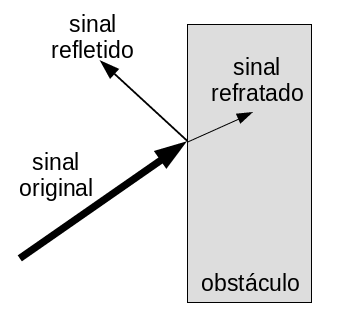
\includegraphics[scale=0.4]{img/reflexao.png}\label{fig:mecprop:a}}
	\subfigure[b][Difração]{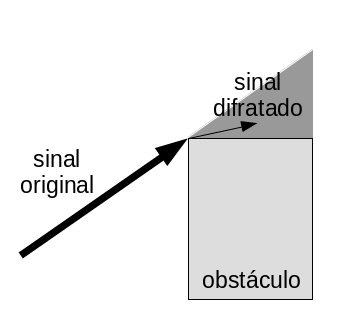
\includegraphics[scale=0.4]{img/difracao.png}\label{fig:mecprop:b}}
	\subfigure[c][Dispersão]{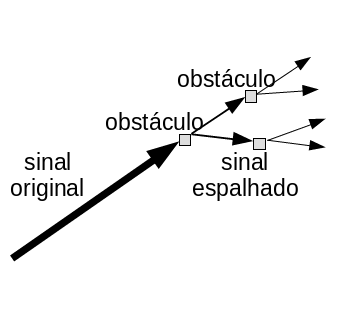
\includegraphics[scale=0.4]{img/espalhamento.png}\label{fig:mecprop:c}}
	\caption{Mecanismos de propagação.}
	\label{fig:mecprop}
\end{figure}

\begin{itemize}
\item Reflexão e refração: 
A figura \ref{fig:mecprop:a} mostra o que acontece quando o sinal propagado em um meio colide com um obstáculo de propriedades diferentes. Parte do sinal original é refletida para o meio e parte é refratada para o obstáculo. \cite{rappaport2009comunicacoes} %conferido
\item Difração:
A difração ocorre quando o sinal incide sobre a extremidade de um obstáculo de dimensões maiores que o comprimento de onda do sinal. Neste caso, como ocorre na figura \ref{fig:mecprop:b}, parte da energia do sinal original é redirecionada para a região de sombra causada pelo obstáculo. \cite{rappaport2009comunicacoes} %conferido
\item Dispersão: 
Como mostra a figura \ref{fig:mecprop:c}, a dispersão ocorre quando a onda de rádio incide sobre muitos obstáculos. Neste caso o sinal original é dividido e desviado em múltiplas direções. \cite{rappaport2009comunicacoes} %conferido
\end{itemize}

\subsubsection{Potência}

O cálculo da potência recebida, em Watts, por uma antena é dado pela equação de Friis (\ref{eq:friis}), onde ${P}_{r}$ é a potência recebida, ${P}_{t}$ é a potência transmitida, ${G}_{t}$ é o ganho da antena de transmissão, ${G}_{r}$ é o ganho da potência de recepção e ${L}_{p}$ é a atenuação no percurso. \cite{rappaport2009comunicacoes} \cite{haykin2009sistemas}

\begin{equation}
{P}_{r} = \frac{{P}_{t}{G}_{t}{G}_{r}} {{L}_{p}}
\label{eq:friis}
\end{equation}

Sabendo que decibél (dB) é uma unidade logarítmica usada para expressar a razão entre duas quantidades físicas e aplicando as propriedades dos logaritmos, a equação \ref{eq:friis} pode ser transformada na equação \ref{eq:friisLog}. \cite{haykin2009sistemas}

\begin{equation}
{P}_{r} = {P}_{t}+{G}_{t}+{G}_{r}-{L}_{p}
\label{eq:friisLog}
\end{equation}

A transformação da potência $P_W$ em W para $P_{dB}$ em dB é dada pela equação \ref{eq:pwdb}, onde $P_0$ é igual a 1W.

\begin{equation}
P_{dB} = 10 \log_{10} \left (\frac{P_W}{P_0} \right )
\label{eq:pwdb}
\end{equation}

A atenuação no percurso, para o espaço livre, em dB, definida conforme a equação \ref{eq:atenucaoEspLivre}, onde $n$ o coeficiente de perda do percurso, $d$ é a distância entre as antenas em metros, $f$ é a frequência do sinal em GHz e $c$ é a velocidade da luz em m/s. \cite{haykin2009sistemas}

\begin{equation}
{L}_{p} = n10\log_{10}{\left ( \frac{4\pi df}{c} \right )}
\label{eq:atenucaoEspLivre}
\end{equation}


\subsubsection{Protocolos 802.11}

Redes sem fio são regulamentadas pelo Institute of Electrical and Eletronics Engineers, padrão conhecido como IEEE 802.11, sendo os principais: \cite{tanenbaum2003redes} %conferido%

\begin{description}
\item[IEEE 802.11a] 5GHz, com transferências a até 54Mbps.
\item[IEEE 802.11b] 2.4GHz, com transferências a até 11Mbps.
\item[IEEE 802.11g] 2.4GHz, com transferências a até 54Mbps.
\item[IEEE 802.11n] 2.4 GHz ou 5GHz, com transferências a até 600Mbps.
\item[IEEE 802.11ac] 5GHz, com transferências a até 1Gbps.
\end{description} %conferido%
 
\subsection{Problema de posicionamento para cobertura sem fio}

A implantação de redes sem fio em ambientes internos ou externos demanda a análise de muitas variáveis. Características físico-químicas dos obstáculos e do ambiente, interferências eletromagnéticas e o posicionamento dos pontos de acesso influenciam na qualidade do sinal. A cobertura total de um ambiente depende do número e do posicionamento dos pontos de acesso. \cite {freytag2013desenvolvimento}%conferido%   

\subsubsection{Modelos propagação}

O meio de propagação de um sistema sem fio é o canal de rádio. Suas características e efeitos são de natureza complexa, o que impossibilita uma análise completamente determinística. São utilizados então, dados experimentais. Medições indicam, por exemplo, que as flutuações de pequena escala e larga escala do sinal variam. Esses parâmetros são importantes para a construção de um modelo que retrate a realidade. Existem vários tipos de modelos de propagação. \cite{najnudel2004estudo} %conferido%

 Os modelos teóricos não possuem nenhum tipo de ajuste experimental. São baseados na solução da equação da onda onde são consideradas as condições do ambiente e apresentam alto custo computacional. Os modelos semi empíricos são baseados em aproximações estatísticas e testes empíricos para se ajustar à vários tipos de ambientes. São menos exatos, entretanto possuem baixo custo computacional. É importante salientar que todos os modelos derivam da equação de Friis \ref{eq:friisLog} \cite{najnudel2004estudo} %conferido%

O modelo \textit{Log-distance} é o modelo semi-empírico mais simples para a perda de percurso em ambientes fechados. É definido pela equação \ref{eq:log_distance}, ${L}_{total}$ representa a perda total, ${L}_{0}$ a perda inicial.  Os parâmetros $n$ e $\sigma$ podem ser escolhidos para representar diferentes ambientes e faixas de frequência. \cite{najnudel2004estudo}


\begin{equation}
{L}_{total} = {L}_{0} + 10 n \log(d) + {X}_{\sigma}
\label{eq:log_distance}
\end{equation}

O modelo ITU-R P.1238-1, descrito pela equação \ref{eq:itu}, foi desenvolvido pelo setor de radiocomunicação do \textit{International Telecommunication Union} (ITU-R), para medição de sinais na faixa de frequência entre 900MHz e 100GHz em ambientes fechados. Esse modelo considera:

\begin{itemize}
\item Reflexão e difração em objetos físicos.
\item Transmissão através de paredes, pisos e outros obstáculos fixos.
\item Confinamento da energia em corredores.
\item Pessoas e objetos em movimento no ambiente.
\end{itemize}

\begin{equation}
{L}_{total} = 20 \log(f) + n \log(d) + {L}_{f}({k}_{f}) - 28
\label{eq:itu}
\end{equation}

Na equação \ref{eq:itu}, $L_{total}$ é a perda total, $f$ é a frequência de operação em MHz, $n$ é o coeficiente de atenuação com a distância, $d$ é a distância percorrida em metros, $k_f$ é o número de pisos (andares) atravessados e $L_f$ é o coeficiente de atenuação por piso atravessado em dB. O ITU-R fornece o coeficiente de atenuação com a distância para três ambientes e para seis faixas de frequência, como mostra a tabela\ref{tbl:coeficienteDistanciaItu} \cite{najnudel2004estudo}

\begin{table}[ht]
\centering
\caption{Coeficiente de atenuação em relação à distância (ITU-R P.1238-1)}
\label{tbl:coeficienteDistanciaItu}
\begin{tabular}{cc}
\hline
\textbf{Tipo do ambiente} & \textbf{Coeficiente(n)} \\
\hline
Residencial & 28 \\
\hline
Escritório & 30 \\
\hline
Comercial & 22 \\
\hline
\end{tabular}
\end{table}

A recomendação para o coeficiente de atenuação por piso atravessado segue o padrão do coeficiente de atenuação em relação à distância. Como mostra a tabela \ref{coeficientePisoItu}. \cite{najnudel2004estudo}

\begin{table}[ht]
\centering
\caption{Coeficiente de atenuação por piso atravessado (ITU-R P.1238-1)}
\label{tbl:coeficientePisoItu}
\begin{tabular}{cc}
\hline
\textbf {Tipo do ambiente} & \textbf{Coeficiente ($L_t$)}\\ 
\hline
Residencial & $4 k_t$ \\
\hline
Escritório & $15 + (k_f - 1)$ \\
\hline
Comercial & $6 + 3 (k_f - 1)$\\
\hline
\end{tabular}
\end{table}

O modelo ITU-R P.1238-1 representa o valor médio do sinal e não contempla as variações de pequena e larga escala so sinal. No caso de sombreamento, a distribuição utilizada é log-normal, equação \ref{eq:logNormal}, onde $m$ é o valor médio da distribuição em dB e $\sigma$ é o desvio médio padrão da distribuição em dB. \cite{najnudel2004estudo} 

\begin{equation}
{p}_{r}(r) = \frac{1}{\sqrt{2\pi \sigma}}exp\left[-\frac{1}{2} { \left(\frac{r-m}{\sigma}\right)}^{2}\right]
\label{eq:logNormal}
\end{equation}

O modelo COST 231 Keenan e Motley é o mais completo para predição de sinais em ambientes fechados com existência de obstáculos. É um modelo abrangente mas que demanda muitos dados, representado pela equação \ref{eq:cost231}. O ${L}_{0}$ é a perda de propagação a um metro da antena irradiante (dB), $d$ é a distância percorrida pelo sinal (m), $n$ é o coeficiente de propagação, ${L}_{f,i}$ é a perda de propagação do sinal através do piso \textit{i} (dB), ${k}_{f,i}$ é o número de pisos com a mesma característica, ${L}_{w,i}$ é a perda de propagação do sinal através da parede \textit{j} (dB), ${k}_{f,i}$ é o número de pisos com a mesma característica, I é o número de pisos atravessados pelo sinal e J é o número de paredes atravessados pelo sinal. \cite{najnudel2004estudo}

\begin{equation}
{L}_{total} = {L}_{0} + 10 n \log (d) + \sum_{i=1}^{I} ({k}_{f,i} {L}_{f,i}) + \sum_{j=1}^{J} ({k}_{w,i} {L}_{w,i})
\label{eq:cost231}
\end{equation} 

Alguns dos valores obtidos experimentalmente são mostrados na tabela \ref{tbl:coeficienteDistanciaKenMot}:

\begin{table}[ht]
\centering
\caption{Coeficiente de perda no percurso para vários ambientes (COST 231 Keenan e Motley)}
\label{tbl:coeficienteDistanciaKenMot}
\begin{tabular}{cc}
\hline
\textbf{Tipo do ambiente} & \textbf{Coeficiente(n)}\\ 
\hline
 Espaço livre & 2\\
\hline
Interno, salas de aula  & 1.2\\ 
\hline
Interno, lab de informática & 1.4\\
\hline
\end{tabular}
\end{table}

\section{Métodos de solução de problemas complexos}

Há duas maneiras de solucionar um problema complexo: métodos heurísticos e o método exaustivo. É necessária uma análise individual para determinar qual o método mais adequado para solucionar um problema. \cite{junior2008proposta} %conferido

\subsection{Método exaustivo}

Também chamado de solução por força bruta, tem como objetivo analisar absolutamente todos os cenários possíveis para decidir se existe uma solução ótima para o problema e qual ela é. Após analisar todos os cenários possíveis de um problema, pode-se afirmar com certeza que o algoritmo encontrou a solução ótima. A vantagem desse método é encontrar a resposta ótima. A grande desvantagem é o alto custo computacional, que devido ao tempo necessário para percorrer todos os estados. \cite{junior2008proposta} %conferido

\subsection{Métodos heurísticos}

Os métodos heurísticos se utilizam de regras, estratégias, procedimentos, métodos de aproximação, tentativa/erro, para a procura da melhor solução de um problema. Por não analisar todos os estados possíveis para encontrar uma solução, os processos heurísticos exigem menos custo computacional que o método exaustivo. Eles são mais próximos da forma como o ser humano raciocina e chega às soluções eficientes. \cite {junior2008proposta} %conferido

É importante ressaltar as vantagens e desvantagens da utilização dos métodos. O método exaustivo garante encontrar a solução ótima a um custo computacional alto. O método heurístico não garante encontrar a solução ótima, porém encontra soluções de boa qualidade com um custo computacional aceitável. \cite{luke2009metaheuristics} %conferido

Exitem heurísticas que iterativamente trabalham com uma única solução. \textit{Hill Climbing} é um exemplo deste tipo de heurística. Existem também heurísticas que trabalham com conjuntos de soluções por iteração. Como exemplo deste tipo de heurística, os Algorítmos genéticos. \cite{luke2009metaheuristics}%conferido  

\subsubsection{Hill Climbing}

É uma técnica relacionada com um gradiente ascendente. Não requer conhecimento sobre o tamanho, nem sobre a direção desse gradiente. É necessário testar iterativamente novas soluções candidatas na vizinhança da solução atual e substituir a atual pela candidata quando a solução candidata é melhor. Isto permite uma subida até o ótimo local. O algoritmo apresenta baixo custo computacional, porém é pouco eficiente em relação à encontrar uma melhora para a solução. \cite{luke2009metaheuristics} %conferido

\subsubsection{Algoritmos Genéticos}

O algoritmo genético é uma heurística populacional baseada na ideia da evolução das espécies. As soluções candidatas são tratadas como indivíduos e as variáveis das soluções como genes. Parte da premissa de que os indivíduos mais aptos tem mais sucesso em repassar as suas características para a geração seguinte. Desta forma, as melhores soluções de uma iteração são misturadas na expectativa de gerar soluções cada vez melhores para a próxima iteração. Assim como na natureza, também é utilizado o conceito de mutação, na qual o valor de uma variável é alterado. \cite{luke2009metaheuristics} \cite{mitchell1998introduction} %conferido

\begin{lstlisting}[caption=Algoritmo genético canônico, label=algGeneticoCan]
inicialize a populacao atual aleatoriamente
avalie a qualidade dos individuos da populacao atual
repita
	enquanto nova populacao nao estiver completa
		escolha pai e mae segundo algum criterio de selecao
		gere dois filhos por cruzamento
		cause mutacoes nos filhos
		adicione os filhos na nova populacao
	fim
	avalie a qualidade dos individuos da nova populacao
	copie os individuos da nova populacao para a atual
ate que o criterio de satisfacao seja satisfeito
\end{lstlisting}

O algoritmo \ref{algGeneticoCan} começa inicializando todas as variavéis que formam as soluções candidatas. A avaliação da qualidade de uma solução candidata é feita com base no valor em suas variáveis. É com base na evolução da qualidade do indivíduos que se resolve o problema. O cálculo da qualidade também engloba as restrições às quais o problema está sujeito. O processo de escolha de pai e mãe efetua a seleção de soluções candidatas para gerar as soluções da próxima geração. Ajustada corretamente, é esta operação que conduz a população de soluções candidatas para regiões mais promissoras do espaço de busca. Roleta e torneio, são os tipos mais usados de seleção. O processo de cruzamento envolve gerar dois filhos a partir do pai e da mãe selecionados anteriormente. Neste processo, genes dos pais são misturados de modo que cada filho herde características de ambos. Cruzamento em um ponto, cruzamento em dois pontos e cruzamento uniforme são alguns tipos de cruzamento. O próximo passo é a mutação. Significa alterar probabilisticamente o valor de alguns dos genes que compõe o indivíduo. Por fim, os indivíduos da nova geração se tornam a geração atual e o processo se repete até que o critério de satisfação seja satisfeito. Alguns critérios de satisfação utilizados são número máximo de iterações e convergência da população. \cite{luke2009metaheuristics} \cite{mitchell1998introduction} %conferido


%\subsection{Objetivo}

%OBJETIVO 

%\subsection{Tipos (SISD,SIMD,MISD,MIMD)}

%TIPO

%\subsection{Formas}

%FORMAS

%\subsubsection{Memória compartilhada}

%MEMORIA COMPARTILHADA

%\subsubsection{Troca de Mensagens}

%TROCA DE MENSAGENS

\chapter{Trabalhos relacionados} 

A otimização do posicionamento de pontos de acesso para melhoria de cobertura de redes sem fio, utilizando algoritmo genético, é encontrada nos três seguintes estudos que servem de referência para este trabalho.

Em \cite{ji2002methods} um algoritmo genético foi desenvolvido para realizar a alocação de pontos de acesso que calcula a quantidade e a posição de cada equipamento, utilizando uma adaptação do modelo COST 231 Keenan e Motley; codificação binária; uma planta hipotética; pontos de acesso com especificação homogênea, configurados para comunicação nos padrões IEEE 802.11b e 802.11g.

Em \cite{vellasco2010dimensionamento} foi desenvolvido um algoritmo genético para calcular a alocação de um número determinado pelo usuário de pontos de acesso, utilizando uma adaptação do modelo COST 231 Keenan e Motley; codificação real; uma planta hipotética; pontos de acesso com especificação homogênea, configurados para comunicação no padrão IEEE 802.11b.

Em \cite{nagy2012global} foram desenvolvidos e comparados os resultados de várias heurísticas de busca para realizar a alocação de um número determinado pelo usuário de pontos de acesso. O algoritmo genético utiliza o modelo COST 231 Keenan e Motley; codificação real; a planta real; pontos de acesso com especificação homogênea; o nível do sinal para calcular a cobertura sem fio, ao invés das taxas de transferência dos modelos IEEE 802.11.

\chapter{Metodologia} 

Abaixo serão descritos diagrama de uso, casos de uso e o funcionamento do cálculo da qualidade do sinal exigido para cada célula. Também são apresentados os protótipos de telas e um exemplo de arquivo de entrada no formato XML.

\section{Diagrama de casos de uso} 

A figura \ref{fig:casosDeUso} representa o diagrama de casos de uso da solução que será proposta neste trabalho. O ator é o usuário que utilizará o programa. Suas ações incluem submeter a planta, procurar solução, ajustar os parâmetros e escolher o método de cálculo.

Na ação de submeter planta, o usuário deverá informar ao programa as características do local que ele pretende efetuar o cálculo. Informações como, posição e densidade de obstáculos e tamanho do local deverão ser inseridas nessa etapa. Ajustar os parâmetros é definir os coeficientes de perda dos obstáculos. Na escolha do método de cálculo, o usuário deverá informar qual é o modelo de perda de sinal que ele deseja utilizar. A ação de procurar solução, é a responsável por aplicar a heurística escolhida e devolver a resposta ao usuário.

\begin{figure}[h]
\centering
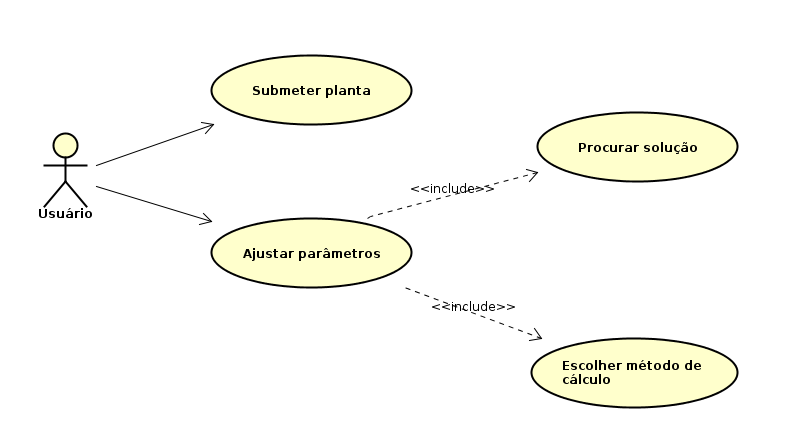
\includegraphics[scale=0.55]{img/casosDeUso.png}
\caption{Diagrama de Casos de Uso}
\label{fig:casosDeUso}
\end{figure}

\section{Diagrama de classes}

A figura \ref{fig:diagramaDeClasses} representa o diagrama de classes da solução proposta. 

A classe AlgoritmoGenetico é a classe responsável pela implementação da heurística. Ela se relaciona com as classes Planta, População, Modelo, Cruzamento, Seleção e Mutação.

Planta é uma classe que representa a planta baixa de um prédio que será submetida pelo usuário. Uma Planta é composta de um ou mais objetos do tipo Paredes. A classe Parede reúne as características das paredes, suas coordenadas e seus coeficientes. 

População é a classe onde está representada as populações, atual e nova, sobre as quais o algoritmo genético irá iterar. Cada população é composta de $n$ indivíduos e cada indivíduo de $k$ genes. 

As classes ITUr e Cost231 implementam a interface Modelo e são responsáveis pelo cálculo da perda de sinal em relação à distância e através dos obstáculos.

A classe Uniforme implementa a interface Mutacao. É ela a responsável por fazer a mutação nos genes dos indivíduos.

As classes Torneio e Roleta implementam a interface Selecao. São estas classes que farão a seleção de pais na população atual para gerar filhos na próxima geração.

As classes UmPonto, DoisPontos e Uniforme são classes que implementam a interface Cruzamento. São as classes que modelam como os genes dos indivíduos selecionados serão mesclados para produzir descendentes na nova população. 

\begin{figure}[h]
\centering
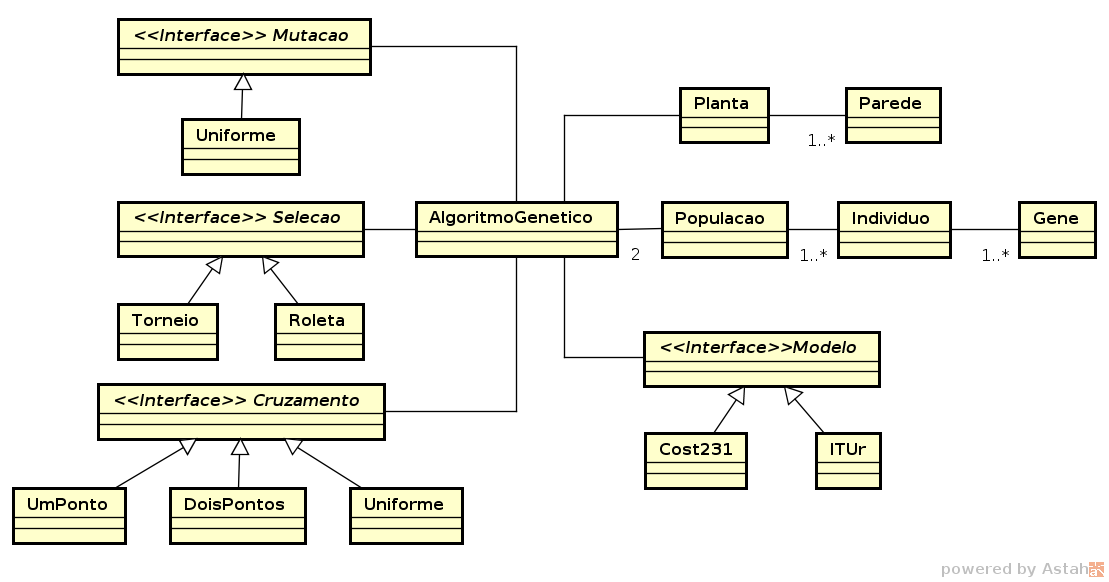
\includegraphics[scale=0.5]{img/diagramaDeClasses.png}
\caption{Diagrama de Classes}
\label{fig:diagramaDeClasses}
\end{figure}

\section{Algoritmo de análise de qualidade}

O algoritmo genético ranqueia as soluções baseado em um critério de qualidade. Para esse processo é necessário que a planta baixa submetida pelo usuário seja dividida em células de acordo com a discretização ajustada pelo usuário. São posicionados então os roteadores e em cada célula é calculado o valor do sinal recebido. Esse cálculo é feito pelo modelo de propagação de sinal escolhido pelo usuário já citados aqui no texto. %conferido%
 
O algoritmo \ref{algCalQual} representa a avaliação da qualidade de cada célula. Para cada célula gerada a partir da planta que o usuário submeter, para cada \textit{access point}, é feito o cálculo do sinal que chega nessa célula de acordo com o modelo escolhido pelo usuário. É escolhido então, o maior dos valores, entre os sinais enviados pelos diversos \textit{access points}. Em seguida, o algoritmo faz a contagem das células que recebem sinal considerado abaixo do aceitável e acima do desejado. Aplica-se os pesos que serão utilizados para definir a qualidade da solução.     

\begin{lstlisting}[caption=Algoritmo cálculo da qualidade canônico, label=algCalQual]
Para cada celula
	Para cada access point
		Calcula potencia celula
	Encontra a potencia maxima dentre os access points
	Converte potencia em taxa de transferencia
Conta celulas abaixo do aceitavel
Conta celulas acima do desejado
Aplica pesos
Obtem qualidade da solucao
\end{lstlisting}

\section{Protótipos de telas}

Como mostra a figura \ref{fig:prototipoUm}, a tela de início possui um espaço para o usuário escolher o arquivo XML que especifica a planta baixa que será analisada. Os botões disponíveis são Submeter, Ajustar parâmetros e Calcular. 
No botão Submeter será aberto uma janela para navegar entre arquivos e selecionar a planta baixa. O botão Ajustar parâmetros abre uma outra tela ilustrada pela figura \ref{fig:prototipoDois}. O botão Calcular, dá início ao procedimento de busca pela solução.

\begin{figure}[!h]
	\centering
	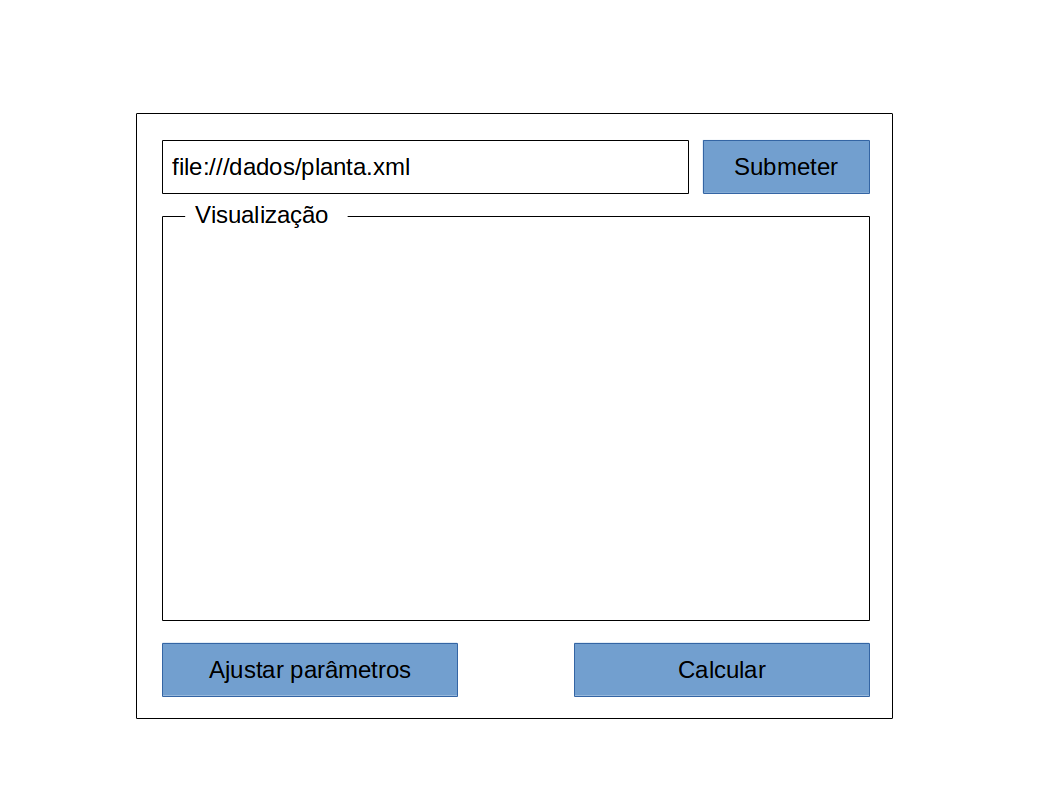
\includegraphics[scale=0.4]{img/prototipo1.png}
	\caption{Protótipo da tela de início do sistema}
	\label{fig:prototipoUm}
\end{figure}

A figura \ref{fig:prototipoDois} ilustra a tela onde os ajustes de parâmetros do sistema serão feitos. Parâmetros como número de gerações utilizadas pelo algoritmo genético, modelo da perda de sinal, coeficiente de perda do ambiente são ajustados nessa etapa. O botão Ajustar salva esses dados e redireciona para a tela ilustrada na \ref{fig:prototipoUm}.

\begin{figure}[!h]
	\centering
	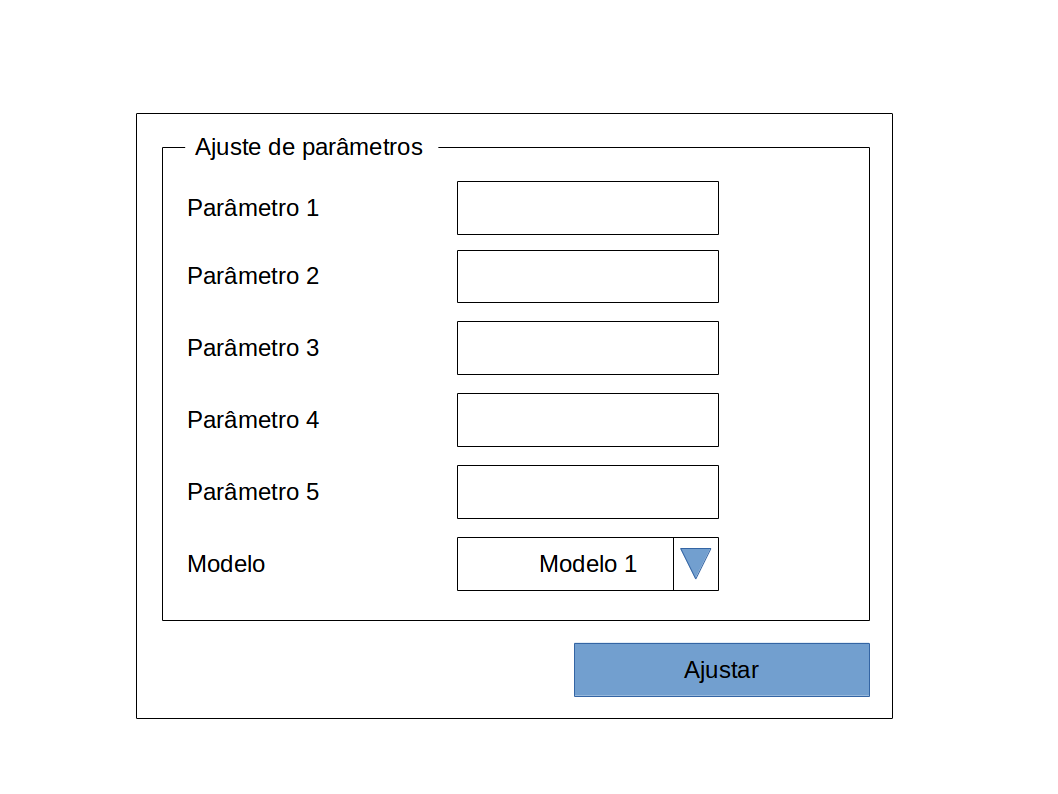
\includegraphics[scale=0.4]{img/prototipo2.png}
	\caption{Protótipo da tela de ajuste de parâmetros}
	\label{fig:prototipoDois}
\end{figure}

A figura \ref{fig:prototipoTres} mostra um rascunho de como será a tela de exibição dos resultados. A principal informação dessa tela será um desenho contendo a planta que foi submetida mostrando a dispersão do sinal através de cores, o número de roteadores que algoritmo vai calcular e suas posições. O botão Exportar, vai guardar esse resultado em um arquivo que possa ser guardado depois. 

\begin{figure}[!h]
	\centering
	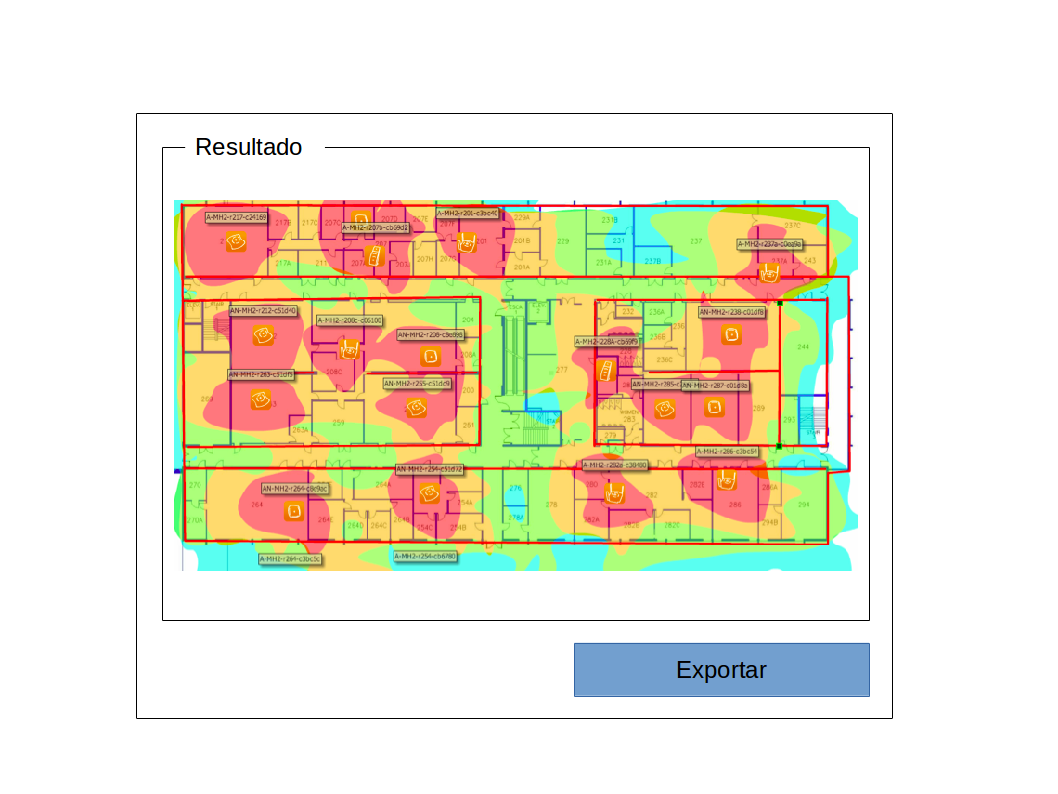
\includegraphics[scale=0.4]{img/prototipo3.png}
	\caption{Protótipo da tela de resultados}
	\label{fig:prototipoTres}
\end{figure}


\section{Tecnologias utilizadas}

A implementação do algoritmo será feita para rodar em um sistema \textit{desktop}. A linguagem utilizada será Java.

\section{Parâmetros do sistema}

Para fazer a análise do local escolhido pelo usuário, o sistema necessita receber como entrada um arquivo XML contendo a descrição da planta baixa que será analisada. Um exemplo desse arquivo é a figura \ref{fig:exemploXml}. Cada planta é composta por $n$ paredes, e cada parede deve conter as seguintes características: deslocamento x e deslocamento y em relação ao canto superior esquerdo da planta, altura, largura e o coeficiente de perda de sinal para aquela parede. 

\begin{figure}[h]
	\centering
	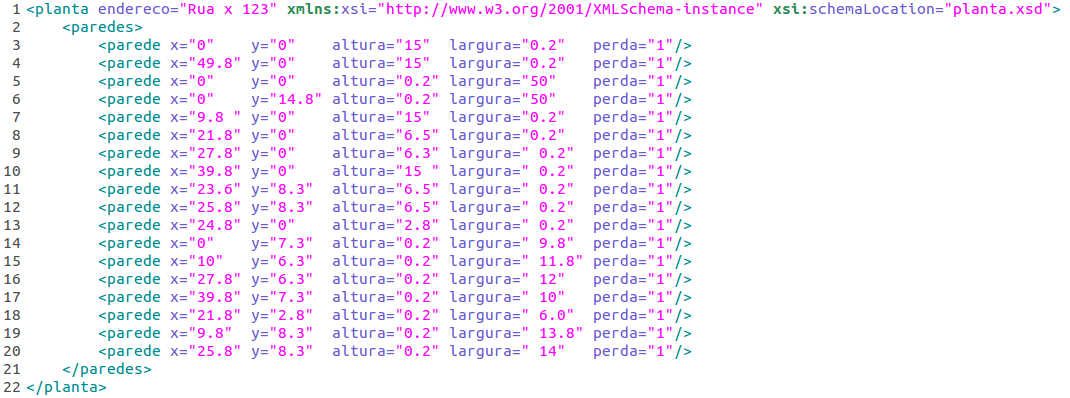
\includegraphics[scale=0.4]{img/exXml.png}
	\caption{Exemplo de arquivo XML}
	\label{fig:exemploXml}
\end{figure}

A figura \ref{fig:exemploXsd} mostra o esquema de validação do arquivo XML submetido com uma planta. 

\begin{figure}[h]
	\centering
	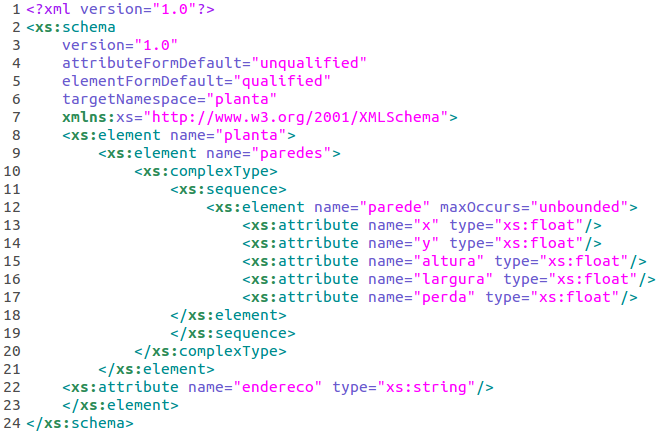
\includegraphics[scale=0.5]{img/exXsd.png}
	\caption{Arquivo XSD de validação da planta}
	\label{fig:exemploXsd}
\end{figure}

A planta baixa representada pelo XML da figura \ref{fig:exemploXml} é apresentada na figura \ref{fig:desenhoPlantaBaixa}.

\begin{figure}[!h]
	\centering
	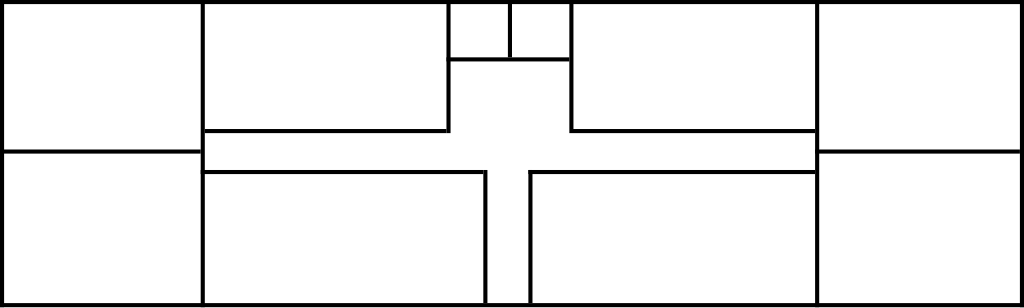
\includegraphics[scale=0.4]{img/plantaBaixaExemplo.png}
	\caption{Desenho da planta baixa}
	\label{fig:desenhoPlantaBaixa}
\end{figure}

	
\chapter{Resultados} 

RESULTADOS

\chapter{Conclusão} 

CONCLUSÃO

\bibliography{bibliografia} 

\chapter*{Glossário} 

\begin{description} 
	\item[\textit{wireless}] tecnologia que não utiliza cabos.
\end{description} 

%\appendix 

%\chapter{APÊNDICE} 

\end{document} 
